% ============================================================================================
% BAB III ANALISIS MASALAH
% Pembagian subbab tidak rigid dan dapat bervariasi. Bab ini minimal berisi analisis kebutuhan
% fungsional dan nonfungsional, analisis berbagai alternatif solusi yang dapat ditawarkan, dan
% metode pemilihan solusi yang diusulkan.
% ============================================================================================
\cleardoublepage
\chapter{ANALISIS MASALAH}
\label{chap:analisis-masalah}
Bab ini membahas secara mendalam analisis masalah yang terdapat pada sistem manajemen akses fisik saat ini di Gedung ITB Innovation Park (IIP), analisis kebutuhan untuk menyelesaikan masalah tersebut, serta analisis pemilihan solusi teknologi yang diusulkan. Secara garis besar, bab ini menguraikan deskripsi hasil analisis dari persoalan keterisolasian data akses karyawan, penjelasan tentang solusi pengembangan middleware ISAPI dan dashboard web pada level konsep desain, serta penjabaran pendekatan rekayasa perangkat lunak yang dipilih untuk merealisasikan solusi tersebut. Alur pembahasan pada bab ini dibagi ke dalam tiga bagian utama, yaitu analisis kondisi sistem kontrol akses saat ini, identifikasi kebutuhan fungsional dan non-fungsional sistem baru, dan diakhiri dengan analisis penentuan alternatif solusi teknologi yang paling optimal.

\section{Analisis Kondisi Saat Ini}
Pengelolaan akses fisik di Gedung ITB Innovation Park (IIP) saat ini berpusat pada area lobi utama yang merupakan jalur perlintasan utama personel. Berdasarkan hasil survei lapangan, alur operasional dan kondisi sistem kontrol akses saat ini divisualisasikan pada Gambar \ref{fig:diagram_alir_saat_ini} (Diagram Alir Proses Saat Ini) dan dijabarkan sebagai berikut:

\begin{figure}[t]
    \centering
    % 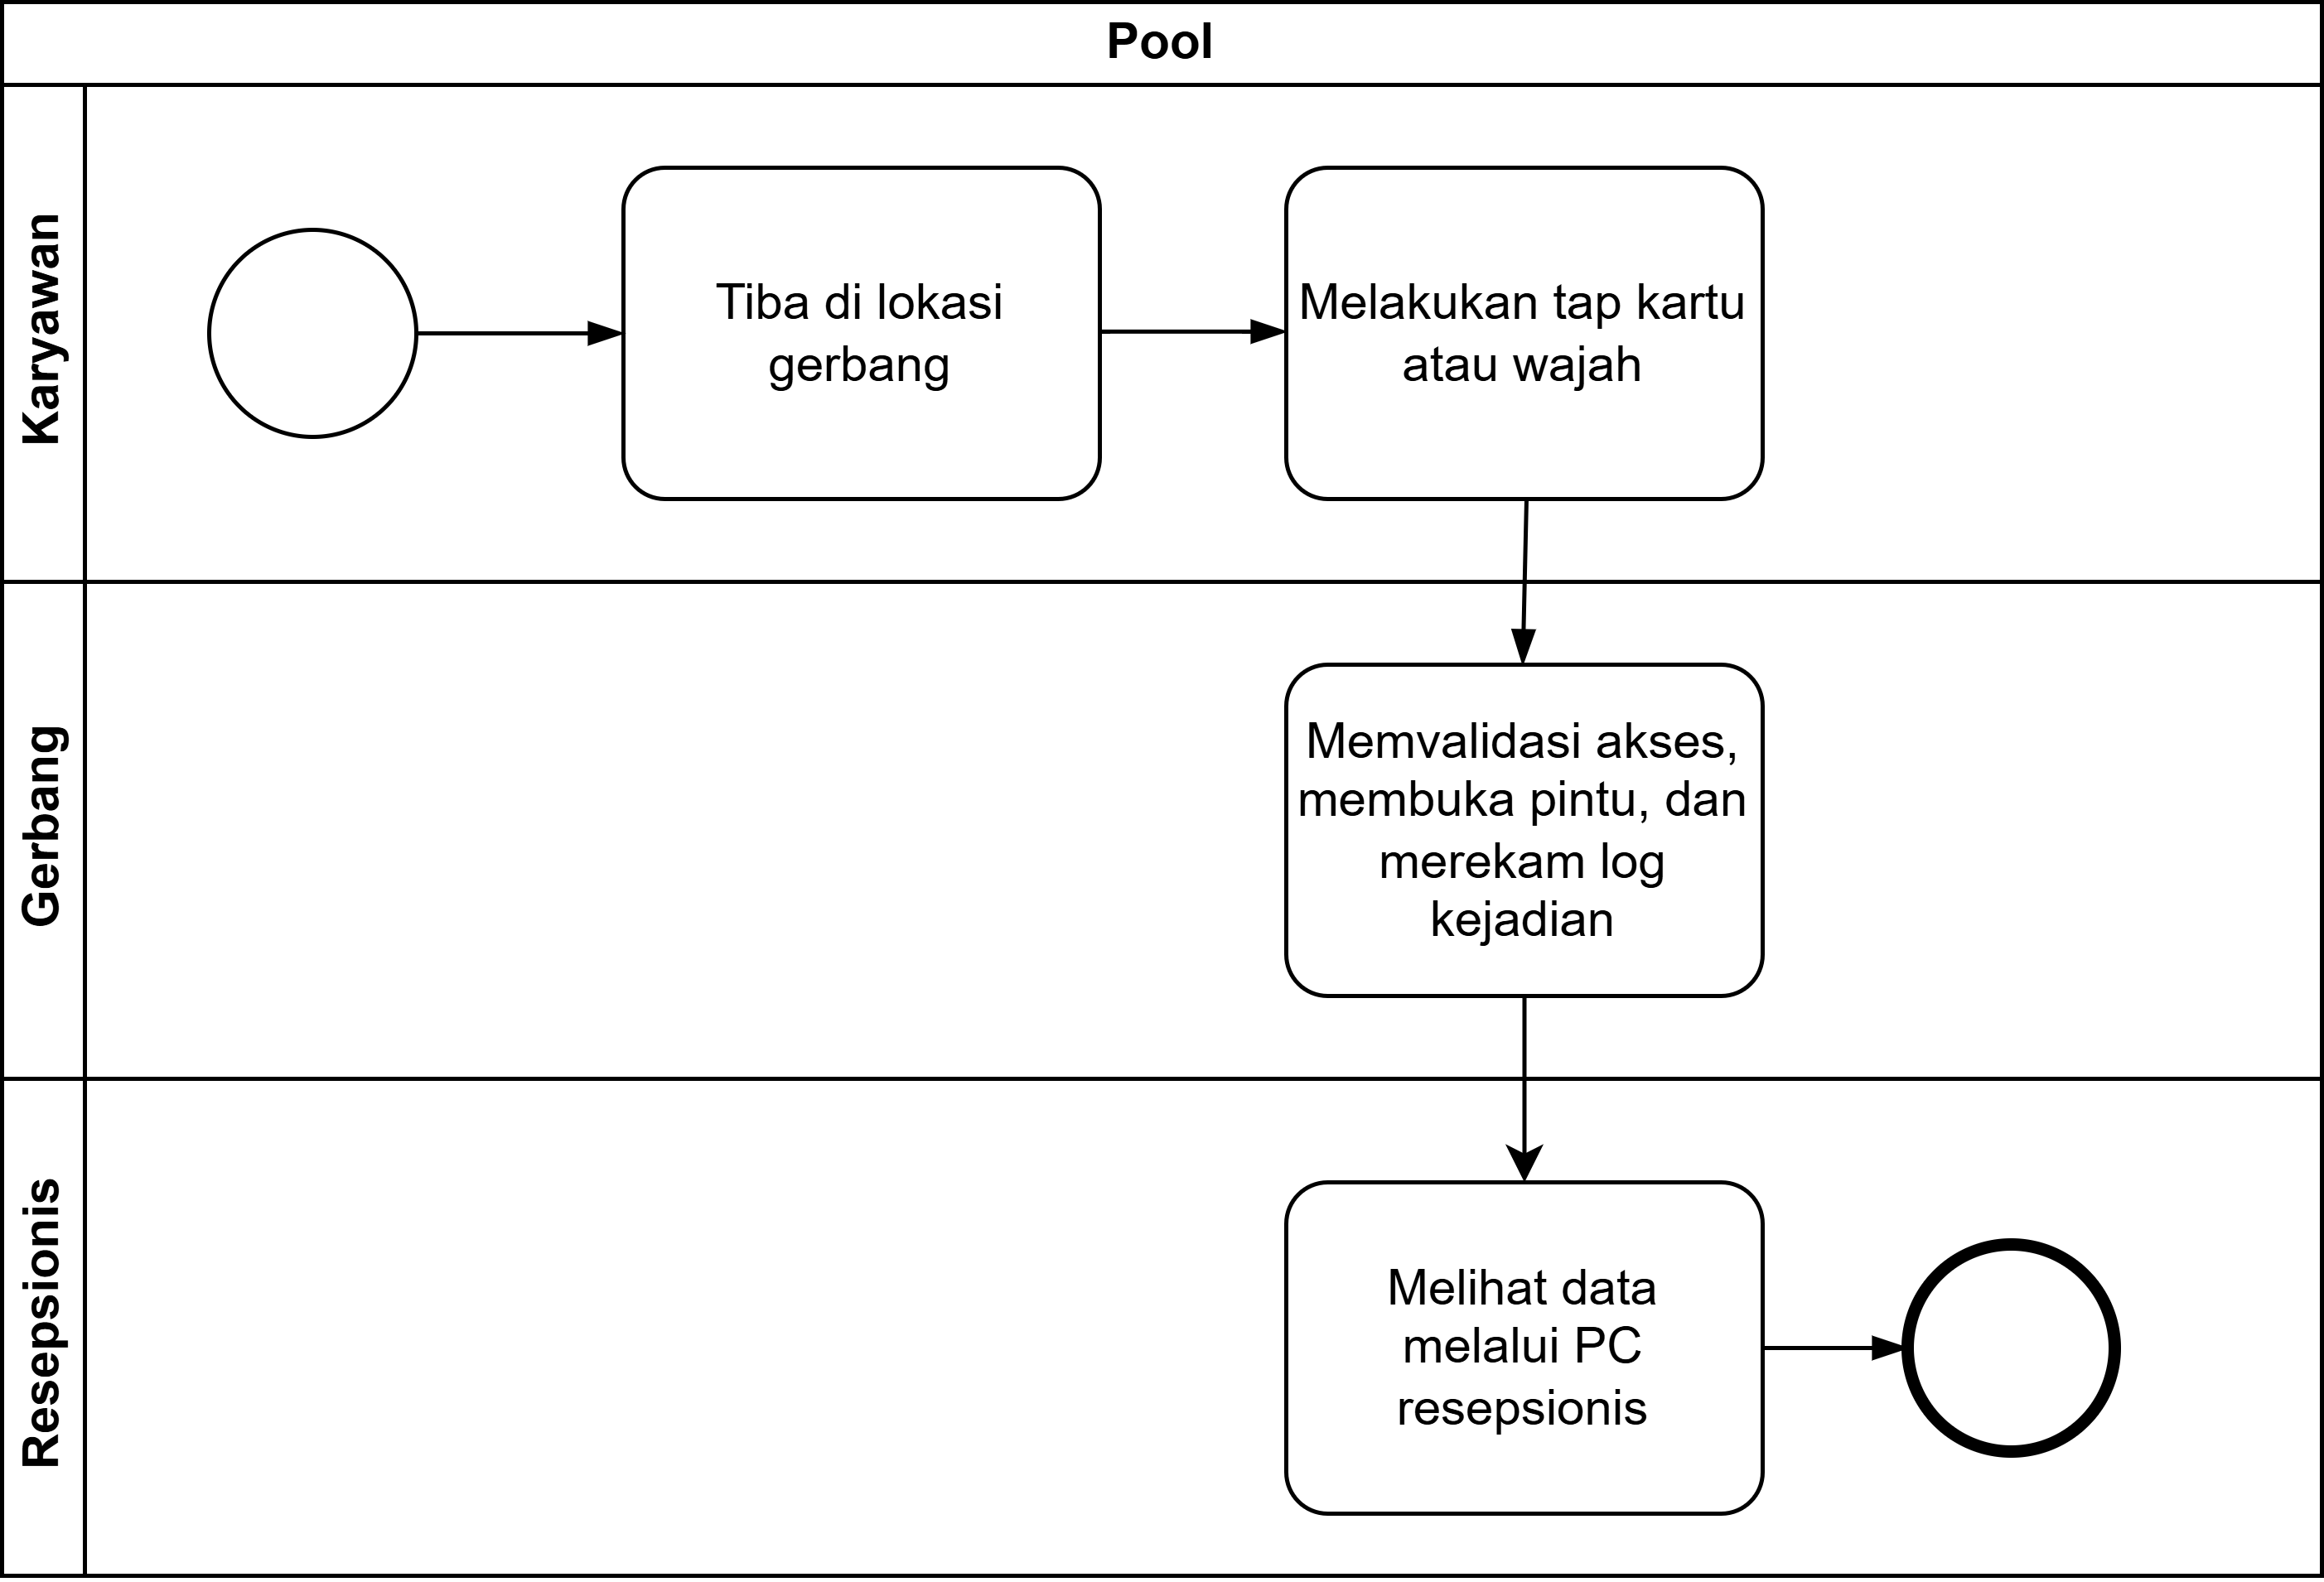
\includegraphics[width=0.8\textwidth]{images/diagram_alir_saat_ini.png}
    \vspace{4cm} % Placeholder untuk Diagram Alir Proses Saat Ini
    \caption{Diagram Alir Proses Manajemen Akses Saat Ini}
    \label{fig:diagram_alir_saat_ini}
\end{figure}

\subsection{Konfigurasi Perangkat Keras di Lobi Utama}
Area lobi dilengkapi dengan tiga jalur (lane) gerbang pembatas. Untuk mendukung fleksibilitas otentikasi, terdapat total 6 (enam) unit terminal akses biometrik yang terpasang (2 unit per jalur untuk akses masuk dan keluar). Seluruh perangkat tersebut telah mendukung teknologi pemindaian wajah (face recognition), kartu RFID, dan pemindaian sidik jari (fingerprint). Saat ini, terminal-terminal tersebut telah beroperasi normal dan tersinkronisasi secara internal di dalam ekosistem perangkat keras vendor.

\subsection{Arsitektur Pengelolaan Data Saat Ini}
Seluruh 6 terminal di lobi terhubung melalui jaringan LAN lokal ke satu unit komputer di area lobi yang bertindak sebagai PC Resepsionis. Komputer ini menjalankan perangkat lunak proprietary vendor (iVMS-4200) yang berfungsi sebagai server lokal untuk konfigurasi perangkat dan penarikan data log. (Catatan Batasan: Meskipun terdapat akses masuk melalui area basemen menggunakan teknologi sidik jari, area tersebut tidak termasuk dalam ruang lingkup penelitian ini dan tidak diberikan solusi dalam pengembangan sistem pada tugas akhir ini. Fokus penelitian sepenuhnya diarahkan pada integrasi web untuk keenam terminal di area lobi utama).

\subsection{Model Konseptual Sistem Saat Ini}
Mengacu pada teori sistem informasi menurut Laudon dan Laudon (2020), model konseptual sistem saat ini di Gedung IIP memiliki komponen sebagai berikut:
\begin{enumerate}
    \item   Input: Registrasi karyawan dilakukan melalui aplikasi desktop vendor pada PC Resepsionis atau didaftarkan langsung di salah satu terminal gerbang.
    \item   Proses: Pemadanan identitas biometrik dilakukan secara mandiri oleh masing-masing dari 6 terminal gerbang saat personel melakukan akses (tapping).
    \item   Output: Pemberian instruksi pembukaan gerbang elektronik dan penyimpanan log transaksi pada memori internal terminal bersangkutan.
    \item   Penyimpanan (Storage): Data log dari keenam terminal ditarik secara periodik dan disimpan ke dalam basis data lokal di PC Resepsionis yang tidak terhubung dengan jaringan web internal gedung.
\end{enumerate}

\subsection{Identifikasi Masalah Utama}
Berdasarkan analisis alur dan arsitektur di atas, masalah fundamental yang ditemukan pada sistem lobi saat ini adalah:
\begin{enumerate}
    \item Akses Data yang Terisolasi (Silo): Meskipun operasional keenam terminal di lobi sudah berjalan dengan baik, data pergerakan log personel hanya dapat dipantau melalui satu PC Resepsionis di lobi. Pihak manajemen atau unit keamanan gedung tidak memiliki sarana untuk memantau lalu lintas karyawan secara real-time melalui peramban web dari ruangan mereka masing-masing.
    \item Ketergantungan pada Perangkat Lunak Vendor (Vendor Lock-in): Pengelolaan data sepenuhnya bergantung pada aplikasi desktop vendor yang memiliki antarmuk   a kaku. Hal ini menyulitkan upaya kustomisasi pengelolaan data karyawan dan menghambat integrasi log akses ke dalam dashboard manajemen gedung cerdas (Smart Building) yang sedang dikembangkan secara internal oleh pihak IIP.
    \item Kesulitan Investigasi Kejadian Anomali: Ketika terjadi kejadian akses yang ditolak (seperti wajah tidak dikenali), pengelola tidak dapat meninjau bukti rekaman visual (snapshot) kejadian tersebut dari jarak jauh. Investigasi terhadap anomali mengharuskan petugas keamanan untuk memeriksa langsung melalui PC Resepsionis di lobi, yang mana proses ini sangat tidak efisien untuk operasional gedung skala besar.
    \item Kerentanan Keamanan Siber BGC: Arsitektur yang terfragmentasi saat ini memiliki celah kerentanan dalam transit data biometrik. Tanpa adanya lapisan pelindung (\textit{Reverse Proxy}) dan enkripsi standar yang terpusat, pertukaran data antara terminal gerbang dan aplikasi lokal rentan terhadap upaya intersepsi data (\textit{man-in-the-middle attack}) yang melanggar standar keamanan siber Bangunan Gedung Cerdas.
\end{enumerate}

\section{Analisis Kebutuhan}
Analisis kebutuhan merupakan tahapan krusial untuk mendefinisikan apa yang harus dilakukan oleh sistem. Metode yang digunakan dalam analisis kebutuhan ini adalah kombinasi antara wawancara semi-terstruktur dengan pihak pemangku kepentingan (\textit{stakeholders}) dan studi kasus observasional terhadap alur kerja di Gedung ITB Innovation Park (IIP). Hasil dari metode ini kemudian disintesis menjadi kebutuhan pengguna, kebutuhan fungsional, dan kebutuhan non-fungsional.

\subsection{Identifikasi Masalah Pengguna}
Berdasarkan hasil wawancara dengan perwakilan pengelola gedung dan Kepala Seksi Data dan Sistem Informasi dari Direktorat Kawasan Sains dan Teknologi (DKST), kebutuhan utama yang diidentifikasi adalah sebagai berikut:
\begin{enumerate}
    \item Aksesibilitas Data Terpusat: Pengelola mengidentifikasi adanya hambatan dalam memantau lalu lintas karyawan karena data hanya tersedia pada PC lokal di area lobi. Dibutuhkan sebuah sistem berbasis web yang memungkinkan pengelola memantau log pergerakan secara \textit{remote} dari titik mana pun di dalam jaringan gedung.
    \item Manajemen Siklus Hidup Karyawan: Dibutuhkan sarana untuk mengelola identitas karyawan (seperti pendaftaran, pembaruan, atau penghapusan hak akses) yang lebih fleksibel dan terpusat tanpa harus bergantung sepenuhnya pada antarmuka aplikasi \textit{desktop} vendor yang kaku.
    \item Pemantauan Riwayat Akses Karyawan: Pengelola membutuhkan sistem yang mampu menarik dan merekapitulasi data log aktivitas karyawan (\textit{check-in} dan \textit{check-out}) secara terstruktur. Hal ini diperlukan untuk memudahkan pelacakan rekam jejak kehadiran personel secara administratif pada operasional sehari-hari.
    \item Dokumentasi Visual untuk Anomali Akses: Petugas keamanan membutuhkan tangkapan layar otomatis (\textit{snapshot}) dari kamera terminal gerbang ketika terjadi kejadian akses yang ditolak (misalnya wajah tidak terdaftar). Berdasarkan preferensi pengelola terkait privasi karyawan, tampilan visual untuk akses yang berstatus normal (berhasil) pada dasarnya tidak menjadi prioritas utama.
\end{enumerate}

\subsection{Kebutuhan Fungsional}
Kebutuhan fungsional mendefinisikan layanan, fitur, dan fungsionalitas yang wajib disediakan oleh sistem berdasarkan hasil analisis masalah. Berikut adalah rincian spesifikasi kebutuhan fungsional sistem yang telah ditetapkan.

\begin{table}[H]
    \centering
    \caption{Kebutuhan Fungsional Sistem}
    \label{tab:kebutuhan_fungsional_sistem}
    \begin{tabular}{|c|p{12cm}|}
        \hline
        \textbf{ID} & \textbf{Deskripsi Kebutuhan Fungsional} \\
        \hline
        KF-01 & Sistem harus menyediakan antarmuka web bagi pengelola untuk memanajemen data profil dan kredensial karyawan (\textit{Create, Read, Update, Delete}). \\
        \hline
        KF-02 & Sistem harus melakukan ekstraksi dan penarikan data riwayat akses (\textit{log}) dari terminal gerbang secara otomatis dan berkesinambungan. \\
        \hline
        KF-03 & Sistem harus memiliki mekanisme sinkronisasi latar belakang (\textit{background process}) untuk memastikan konsistensi data identitas antara peladen dan memori gerbang secara periodik. \\
        \hline
        KF-04 & Sistem harus mampu menyajikan pembaruan status gerbang dan log aktivitas terbaru pada antarmuka \textit{dashboard} secara \textit{real-time}. \\
        \hline
        KF-05 & Sistem harus mampu mengunduh dan menyimpan foto \textit{snapshot} secara otomatis dari terminal gerbang khusus untuk kejadian akses yang ditolak (anomali). \\
        \hline
        KF-06 & Sistem harus menyediakan fitur ekspor data riwayat pergerakan karyawan ke dalam format dokumen (CSV) berdasarkan rentang waktu yang ditentukan. \\
        \hline
    \end{tabular}
\end{table}

\subsection{Kebutuhan Non-Fungsional}
Kebutuhan non-fungsional mendefinisikan batasan, kriteria kualitas, dan atribut performansi yang harus dipenuhi oleh sistem agar dapat beroperasi secara optimal, aman, dan andal. Berikut adalah rincian spesifikasi kebutuhan non-fungsional sistem yang dirangkum pada Tabel \ref{tab:kebutuhan_nonfungsional_sistem}.

\begin{table}[H]
    \centering
    \caption{Kebutuhan Non-Fungsional Sistem}
    \label{tab:kebutuhan_nonfungsional_sistem}
    \begin{tabular}{|c|l|p{9cm}|}
        \hline
        \textbf{ID} & \textbf{Parameter} & \textbf{Deskripsi Kebutuhan Non-Fungsional} \\
        \hline
        KNF-01 & Integritas Data & Transmisi sinkronisasi data harus memiliki tingkat kehilangan (\textit{data loss rate}) mendekati 0\% untuk menjamin konsistensi data presensi harian. \\
        \hline
        KNF-02 & Keamanan & Komunikasi data (API) wajib menggunakan protokol standar (HTTP/ISAPI) dengan metode perlindungan kredensial (\textit{Digest Authentication}). \\
        \hline
        KNF-03 & Auditabilitas & Sistem harus mengakomodasi penyimpanan data visual (\textit{snapshot}) untuk setiap rekam kejadian akses secara utuh guna memfasilitasi validasi akurasi dan audit sistem yang komprehensif. \\
        \hline
        KNF-04 & Aksesibilitas & Aplikasi \textit{dashboard} harus dapat diakses secara fleksibel menggunakan peramban web standar melalui jaringan lokal gedung. \\
        \hline
    \end{tabular}
\end{table}

\section{Analisis Pemilihan Solusi}
Pemilihan solusi teknologi untuk sistem manajemen akses karyawan dilakukan melalui proses evaluasi berlapis terhadap berbagai alternatif komponen arsitektur perangkat lunak. Proses ini bertujuan untuk menentukan kombinasi teknologi yang paling optimal guna menjamin performa penarikan data, integritas basis data, dan kemudahan pemeliharaan sistem.

\subsection{Alternatif Solusi Berdasarkan Komponen Sistem}
Berdasarkan hasil diskusi teknis pada tahap \textit{Ideate}, dilakukan analisis perbandingan terhadap enam komponen utama arsitektur sistem. Setiap komponen dievaluasi menggunakan matriks keputusan dengan parameter bobot yang disesuaikan pada kebutuhan operasional Gedung IIP. Pemberian skor dan pembobotan kriteria pada setiap matriks di bawah ini dilakukan secara kualitatif berdasarkan hasil diskusi tim teknis, evaluasi empiris terhadap dokumentasi resmi masing-masing teknologi, serta pengujian prototipe awal (\textit{Proof of Concept}) pada lingkungan pengembangan.

\subsubsection{API Gateway dan Keamanan}
Evaluasi dilakukan untuk menentukan lapisan pintu gerbang API yang mampu menangani beban lalu lintas layanan dan otentikasi. Berdasarkan Tabel \ref{tab:matriks_api_gateway}, NGINX dipilih karena keunggulannya dalam penggunaan sumber daya yang rendah dan memiliki komunitas dukungan yang sangat luas.
\begin{table}[H]
    \centering
    \caption{Matriks Keputusan Pemilihan API Gateway \& Security Layer}
    \label{tab:matriks_api_gateway}
    \begin{tabular}{|l|c|c|c|c|}
        \hline
        \textbf{Kriteria} & \textbf{Bobot} & \textbf{Kong} & \textbf{NGINX} & \textbf{Traefik} \\
        \hline
        Fitur Keamanan & 30\% & 5 & 4 & 4 \\
        \hline
        \textit{Resource Usage} & 30\% & 3 & 5 & 4 \\
        \hline
        Kemudahan Konfigurasi & 20\% & 3 & 4 & 5 \\
        \hline
        Komunitas/Dukungan & 20\% & 5 & 5 & 4 \\
        \hline
        \textbf{Total Skor} & \textbf{100\%} & \textbf{4.20} & \textbf{4.50}* & \textbf{4.20} \\
        \hline
    \end{tabular}
    \begin{flushleft}
        \small *Dipilih sebagai solusi akhir dalam tahap revisi arsitektur.
    \end{flushleft}
\end{table}

\subsubsection{Layanan Backend dan Logika Bisnis}
Pemilihan kerangka kerja \textit{backend} difokuskan pada kemampuan menangani banyak koneksi terminal secara asinkron. Berdasarkan Tabel \ref{tab:matriks_backend}, NestJS dipilih karena arsitektur modularnya yang memungkinkan pengembangan layanan yang sangat terstruktur dan efisien serta mendukung fungsionalitas seperti \textit{websocket} dan \textit{cron job} yang dibutuhkan oleh sistem yang akan dikembangkan.
\begin{table}[H]
    \centering
    \caption{Matriks Keputusan Pemilihan Backend Dashboard Service}
    \label{tab:matriks_backend}
    \begin{tabular}{|l|c|c|c|c|}
        \hline
        \textbf{Kriteria} & \textbf{Bobot} & \textbf{NestJS} & \textbf{Spring Boot} & \textbf{Golang} \\
        \hline
        \textit{I/O Performance} & 35\% & 5 & 4 & 5 \\
        \hline
        Modularitas & 25\% & 5 & 5 & 3 \\
        \hline
        \textit{Development Speed} & 25\% & 5 & 3 & 4 \\
        \hline
        Ekosistem Library IoT & 15\% & 4 & 4 & 3 \\
        \hline
        \textbf{Total Skor} & \textbf{100\%} & \textbf{4.90} & \textbf{4.00} & \textbf{4.05} \\
        \hline
    \end{tabular}
\end{table}

\subsubsection{Mekanisme Sinkronisasi Data}
Mekanisme ini krusial untuk menjaga konsistensi antara perangkat keras dan server. Berdasarkan Tabel \ref{tab:matriks_sync_engine}, \textit{cron job} dipilih dengan pertimbangan kemudahan implementasi serta efisiensi sumber daya.
\begin{table}[htbp]
    \centering
    \caption{Matriks Keputusan Pemilihan Mekanisme Sinkronisasi Data}
    \label{tab:matriks_sync_engine}
    \begin{tabularx}{\textwidth}{|l|X|X|}
        \hline
        \textbf{Solusi} & \textbf{Kelebihan} & \textbf{Kekurangan} \\
        \hline
        RabbitMQ & Mendukung mekanisme \textit{retry} dan sistem \textit{routing} pesan yang fleksibel, sangat efektif untuk menangani proses asinkron yang membutuhkan keandalan pengiriman data. & Memerlukan instalasi dan pengelolaan \textit{service message broker} tambahan, serta menambah kompleksitas arsitektur dibandingkan solusi bawaan sistem operasi. \\
        \hline
        Apache Kafka & Dirancang untuk \textit{streaming} data bervolume besar dengan tingkat \textit{throughput} yang sangat tinggi serta memiliki toleransi kesalahan (\textit{fault tolerance}) yang superior. & Prosedur instalasi dan pemeliharaan infrastruktur sangat kompleks serta membutuhkan alokasi sumber daya server yang signifikan. \\
        \hline
        Cron Job & Sangat efisien karena merupakan fitur bawaan sistem operasi, ringan, dan tidak memerlukan dependensi eksternal. Sangat ideal untuk kebutuhan \textit{batch processing} atau sinkronisasi berkala. & Tidak bersifat \textit{real-time} (bergantung pada interval penjadwalan) dan memiliki keterbatasan dalam pemantauan otomatis jika terjadi kegagalan proses tanpa integrasi \textit{tooling} tambahan. \\
        \hline
    \end{tabularx}
\end{table}

\subsubsection{Manajemen Basis Data}
Akurasi pencatatan penghuni yang berada di dalam gedung sangat bergantung pada integritas basis data. Berdasarkan Tabel \ref{tab:matriks_database}, PostgreSQL terpilih sebagai solusi mutlak karena kepatuhannya terhadap sifat ACID yang menjamin keamanan data log serta mendukung kebutuhan integritas data yang tinggi.
\begin{table}[htbp]
    \centering
    \caption{Matriks Keputusan Pemilihan Sistem Manajemen Basis Data}
    \label{tab:matriks_database}
    \begin{tabularx}{\textwidth}{|l|X|X|}
        \hline
        \textbf{Solusi} & \textbf{Kelebihan} & \textbf{Kekurangan} \\
        \hline
        PostgreSQL & Menjamin konsistensi data yang tinggi dan mendukung kueri relasional yang kompleks. Memiliki fitur analitik serta mekanisme \textit{indexing} yang sangat mumpuni untuk pengelolaan basis data skala besar. & Prosedur konfigurasi dan optimasi awal relatif lebih kompleks dibandingkan dengan MySQL. \\
        \hline
        MySQL & Memiliki tingkat kemudahan penggunaan yang baik, performa yang stabil untuk aplikasi umum, serta dukungan komunitas yang sangat luas. & Kapabilitas analitik dan fitur kueri tingkat lanjut (\textit{advanced query}) tidak sekomprehensif yang dimiliki oleh PostgreSQL. \\
        \hline
        MongoDB & Menawarkan fleksibilitas tinggi untuk skema data semi-terstruktur serta mendukung skalabilitas horizontal yang efisien melalui mekanisme \textit{sharding}. & Kurang optimal untuk menangani relasi data yang sangat kompleks serta membutuhkan manajemen khusus untuk menjamin konsistensi transaksi tingkat tinggi. \\
        \hline
    \end{tabularx}
\end{table}

\subsubsection{Antarmuka Pengguna (Frontend Dashboard)}
Visualisasi data yang cepat dibutuhkan oleh pihak pengelola dan keamanan saat terjadi kondisi darurat. Berdasarkan Tabel \ref{tab:matriks_frontend}, Next.js memberikan keunggulan berkat fitur \textit{Server-Side Rendering} yang menjamin performa antarmuka tetap responsif.
\begin{table}[H]
    \centering
    \caption{Matriks Keputusan Pemilihan Frontend Dashboard}
    \label{tab:matriks_frontend}
    \begin{tabular}{|l|c|c|c|c|}
        \hline
        \textbf{Kriteria} & \textbf{Bobot} & \textbf{Next.js} & \textbf{React} & \textbf{Vue/Nuxt} \\
        \hline
        Performa SSR & 30\% & 5 & 2 & 5 \\
        \hline
        Ekosistem Komponen & 30\% & 5 & 5 & 4 \\
        \hline
        Kemudahan SEO/Indexing & 20\% & 5 & 2 & 5 \\
        \hline
        \textit{State Management} & 20\% & 5 & 4 & 4 \\
        \hline
        \textbf{Total Skor} & \textbf{100\%} & \textbf{5.00} & \textbf{3.40} & \textbf{4.50} \\
        \hline
    \end{tabular}
\end{table}

\subsubsection{Protokol Komunikasi Antarmuka dan Backend}
Kebutuhan pemantauan instan pada halaman antarmuka dijawab melalui perbandingan pada Tabel \ref{tab:matriks_realtime}. \textit{Websocket} (Socket.IO) beserta RESTful API dipilih sebagai jembatan komunikasi karena kemudahan integrasi dengan ekosistem web modern serta menawarkan perpindahan data yang responsif dan cepat untuk seluruh perangkat yang menjalankan aplikasi.
\begin{table}[H]
    \centering
    \caption{Matriks Keputusan Protokol Komunikasi Real-time}
    \label{tab:matriks_realtime}
    \begin{tabular}{|l|c|c|c|c|}
        \hline
        \textbf{Kriteria} & \textbf{Bobot} & \textbf{Socket.IO} & \textbf{MQTT} & \textbf{REST Polling} \\
        \hline
        Efisiensi Jaringan & 35\% & 4 & 5 & 2 \\
        \hline
        Kemudahan Web Integration & 35\% & 5 & 3 & 5 \\
        \hline
        \textit{Full-Duplex} & 15\% & 5 & 5 & 2 \\
        \hline
        Reliabilitas & 15\% & 5 & 4 & 3 \\
        \hline
        \textbf{Total Skor} & \textbf{100\%} & \textbf{4.65} & \textbf{4.25} & \textbf{3.50} \\
        \hline
    \end{tabular}
\end{table}

\subsubsection{Protokol Komunikasi Perangkat Keras}
Integrasi dengan terminal gerbang Hikvision dilakukan menggunakan protokol ISAPI (\textit{Intelligent Storage Architecture Public Interface}). ISAPI merupakan protokol \textit{native} bawaan perangkat yang berbasis standar HTTP/REST, sehingga bersifat \textit{platform-independent} dan memungkinkan kontrol penuh terhadap fitur-fitur perangkat secara langsung, seperti pengambilan \textit{snapshot} kamera saat terjadi anomali. Penggunaan protokol ini dipilih dibandingkan penggunaan SDK vendor (\textit{HCNetSDK}) untuk menghindari ketergantungan pada sistem operasi tertentu serta meminimalkan beban dependensi eksternal pada aplikasi.

\subsection{Analisis Penentuan Solusi Akhir}
Berdasarkan serangkaian evaluasi terhadap alternatif komponen di atas, diputuskan untuk menggunakan kombinasi solusi akhir sebagai berikut:

\begin{enumerate}
    \item NGINX sebagai API Gateway: Dipilih untuk menangani lapisan keamanan terluar dan \textit{reverse proxy}. NGINX menjamin efisiensi penggunaan sumber daya server dan kemudahan implementasi dibandingkan opsi \textit{message gateway} lainnya.
    \item NestJS sebagai Layanan Backend: Dipilih karena arsitektur modularnya yang memudahkan pemisahan logika antara setiap fungsionalitas dalam \textit{backend}. Teknologi ini juga mendukung fungsionalitas seperti \textit{websocket} dan \textit{cron job} yang dibutuhkan oleh sistem.
    \item Cron Jobs sebagai Sync Engine: Dipilih demi menyederhanakan infrastruktur fisik. Penjadwalan periodik dianggap cukup untuk memenuhi kebutuhan sinkronisasi pada lingkungan lokal Gedung IIP.
    \item PostgreSQL dan Prisma ORM: Dipilih untuk menjamin integritas relasional antara profil karyawan dan log pergerakan penghuni, serta mempercepat pengembangan melalui pemodelan data yang tipe-aman (\textit{type-safe}).
    \item Next.js sebagai Frontend Dashboard: Dipilih untuk memberikan performa antarmuka yang cepat melalui mekanisme \textit{Server-Side Rendering} (SSR), sehingga penyajian data tetap responsif.
    \item Websocket (Socket.IO) dan RESTful API untuk Komunikasi Real-time: Dipilih sebagai jembatan komunikasi dua arah yang memungkinkan pergerakan data muncul di \textit{dashboard} secara instan tanpa pemuatan ulang halaman, memungkinkan petugas keamanan bekerja secara paralel.
    \item Integrasi Protokol ISAPI secara Langsung: Implementasi dilakukan menggunakan protokol bawaan perangkat untuk menjamin sifat \textit{platform-independent} serta memungkinkan kontrol penuh terhadap fitur perangkat keras tanpa ketergantungan pada pustaka SDK vendor yang bersifat spesifik terhadap sistem operasi tertentu.
\end{enumerate}